\section{Descripción del Funcionamiento}

\subsection{Flujo Operativo de la Práctica}
El sistema opera en ciclo continuo sin funciones bloqueantes (\texttt{millis()}):
\begin{enumerate}
    \item \textbf{Inicialización:} Al encenderse, el ESP32 inicializa el bus I²C, el sensor y la salida del LED (\texttt{LOW} por defecto). Establece conexión con el punto de acceso Wi-Fi y con el broker Mosquitto.
    \item \textbf{Telemetría periódica (2 segundos):} Cada $2000\,\text{ms}$, el ESP32 lee la temperatura ($^\circ\text{C}$) y humedad ($\%$) y las publica en los tópicos independientes \texttt{sensor/sht41/temperatura} y \texttt{sensor/sht41/humedad}.
    \item \textbf{Visualización en Dashboard:} Node-RED recibe las lecturas y las representa en tiempo real en los medidores radiales (\textit{gauges}) e historiales gráficos.
    \item \textbf{Control de Actuador (Lazo Cerrado):} El usuario activa el interruptor en el Dashboard; Node-RED envía \texttt{"ON"} a \texttt{actuador/led/set}. El ESP32 recibe la orden, enciende el LED físico en \texttt{GPIO 2} y publica la confirmación \texttt{"ON"} en \texttt{actuador/led/estado}.
\end{enumerate}

\subsection{Ciclo de Control con Confirmación de Estado}
Para evitar que la interfaz muestre estados erróneos si el dispositivo pierde conexión o energía, el switch de Node-RED está configurado en modo \textbf{desacoplado}: la perilla gráfica solo cambia de posición cuando el ESP32 devuelve la confirmación física, como se describe en la Figura~\ref{fig:ciclo_control}.

\begin{figure}[H]
    \centering
    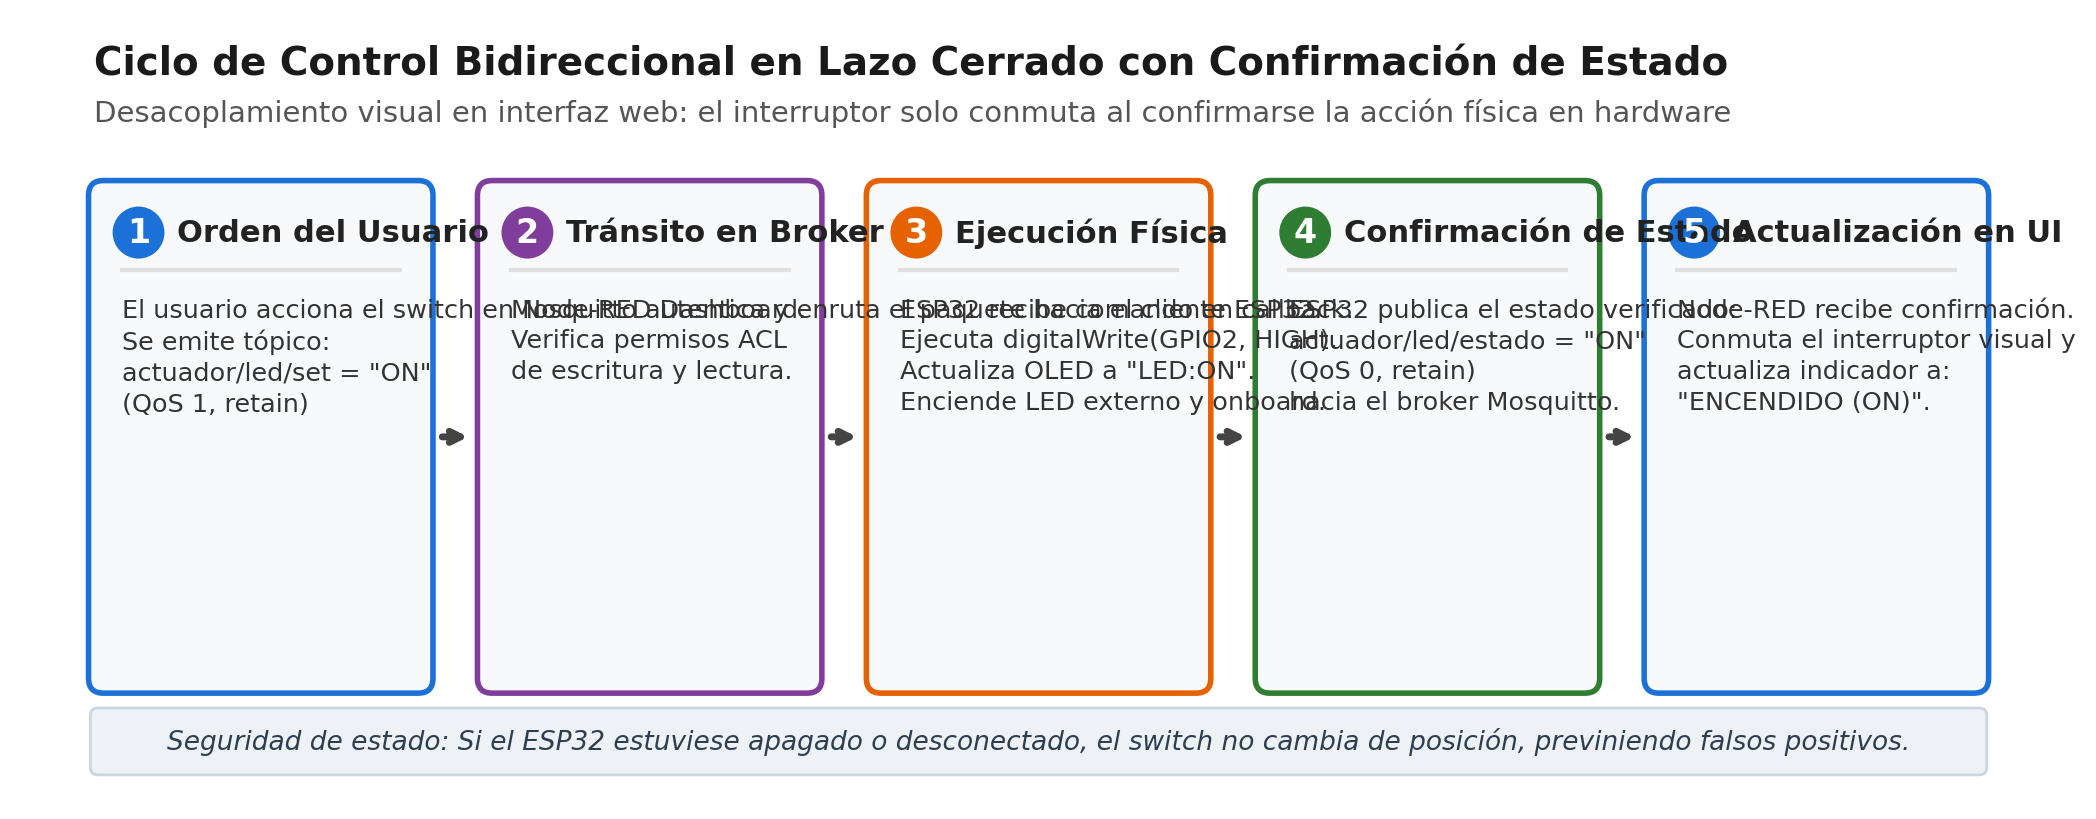
\includegraphics[width=0.96\textwidth]{imagenes/ciclo_control_closed_loop.png}
    \caption{Secuencia de control bidireccional en lazo cerrado con confirmación y desacoplamiento.}
    \label{fig:ciclo_control}
\end{figure}

\subsection{Supervisión de Disponibilidad mediante LWT (\textit{Last Will and Testament})}
\begin{itemize}[noitemsep]
    \item \practicaBadge \textbf{Detección de desconexión:} Al conectarse, el microcontrolador registra en Mosquitto el mensaje \texttt{esp32/status = "offline"} como última voluntad. Una vez enlazado, publica \texttt{"online"}.
    \item Si el ESP32 sufre un corte de energía o pierde señal por más de $1.5 \times \text{keepalive} \approx 22\,\text{s}$, el broker publica automáticamente \texttt{"offline"}. Node-RED detecta el cambio, muestra el estado \textbf{🔴 Desconectado} y despliega una notificación de alerta.
    \item \proyectoBadge \textbf{Visualización local y retención:} La pantalla OLED refleja de inmediato el estado del LED (\texttt{LED:ON} / \texttt{LED:OFF}). Al reconectar tras un reinicio, el ESP32 lee el comando retenido en el broker y restaura el estado del actuador sin intervención del usuario.
\end{itemize}
